%%%%%%%%%%%%%%%%%%%%%%%%%%%%%%%%%%%%%%%%%%%%%%%%%%%%%%%%%%
%%
%% MARK: Title
%%
%%%%%%%%%%%%%%%%%%%%%%%%%%%%%%%%%%%%%%%%%%%%%%%%%%%%%%%%%%

\chapter*{\S B1. Diffeology and Non-Commutative Geometry}
\setcounter{footnote}{0}

%%%%%%%%%%%%%%%%%%%%%%%%%%%%%%%%%%%%%%%%%%%%%%%%%%%%%%%%%%
%%
%% MARK: Abstract
%%
%%%%%%%%%%%%%%%%%%%%%%%%%%%%%%%%%%%%%%%%%%%%%%%%%%%%%%%%%%
\begin{abstract}
  In this lecture we show how we can build a bridge between some diffeological spaces and noncommutative geometry,
  such that diffeomorphic spaces give Morita equivalent $C^*$-algebras.
  These spaces are orbifolds,
  generalized by quasifolds,
  regarded as diffeological spaces.
\end{abstract}

%%%%%%%%%%%%%%%%%%%%%%%%%%%%%%%%%%%%%%%%%%%%%%%%%%%%%%%%%%
%%
%% MARK: Introduction
%%
%%%%%%%%%%%%%%%%%%%%%%%%%%%%%%%%%%%%%%%%%%%%%%%%%%%%%%%%%%

The basic ideas,
at the source of the relationship between diffeology noncommutative geometry,
have been introduced in a first paper \cite{IZL18} of the following two papers,
and its results extended in the second one \cite{IZP21}:

$\bullet$ ``Noncommutative geometry and diffeology: The case of orbifolds'',

$\bullet$ ``Quasifolds, diffeology and noncommutative geometry''.

We have seen that the concept of orbifold has been introduced by Ishiro Stake \cite{Sat56,Sat57} as V-manifolds,
and renamed orbifolds by Thurston \cite{Thu78}.
On the other hand,
its generalization to quasifolds was proposed by Elisa Prato \cite{EP01}.

In the paper ``Orbifolds as diffeologies'' \cite{IKZ10} we include the orbifolds in the category \Category{Diffeology}.
In the second paper we give a diffeological definition of ``quasifolds'' that fits correctly the original definition.
Thus,
quasifolds are also included in the category \Category{Diffeology}.
By this inclusive diffeological approach it is obvious that the Elisa Prato quasifolds are a generalization of orbifolds,
which is not necessarily obvious with the specific definitions.
We have then this particular series of full subcategories:
\[
  \text{\{Manifolds\} $\preceq$ \{Orbifolds\} $\preceq$ \{Quasifolds\} $\preceq$ \{Diffeology\}}.
  \]
Then,
we associate a $C^*$-algebra to the orbifold,
or quasifold,
such that diffeomorphic spaces give Morita equivalent $C^*$-algebra,
which is the minimum required.

I insist on the fact that the process of associating a $C^*$-algebra to these categories of spaces is not tautological
as it can be with a direct algebraic approach which contains already in the definition of the category
(based on groupoids or stacks),
the particular property that equivalent structures (groupoids or stacks) give Morita equivalent $C^*$-algebras.
In our case,
we start here a floor below,
if I may say so,
with the geometry of the space,
that is,
its diffeology.

The outline of the construction is as follows:
\begin{enumerate}
  \item Definition of orbifolds and quasifolds in diffeology.
  \item Introduction of charts and atlases that define the structure.
  \item Associate with every atlas a strict generating family and its nebula.
  \item Associate a groupoid over the space with the nebula of each atlas,
  that captures the local structure point by point.
  \item Prove that two different atlases give equivalent groupoids,
  in the algebraic sense,
  which is the minimum required:
  the groupoid [its class] is a diffeological invariant of the space.
  \item Prove that these groupoids are etale and Hausdorff.
  \item Associate a $*$-algebra,
  and a $C^*$-algebra by completion,
  to each of these groupoids,
  according to Jean Renault's construction.
  \item Use a central theorem from Muhly-Renault-Willian,
  proving that two different atlases give Morita equivalent $C^*$-algebras,
  which is the minimum expected.
  \item And finally illustration by two examples:
  the $C^*$-algebra associated with the irrational torus $\Torus_\alpha$,
  and the $C^*$-algebra associated with the quotient $\RR/\QQ$.
\end{enumerate}

In the two cases,
the idea is to associate a \uline{structure groupoid} to these objects and then,
by a now standard procedure,
associate a $C^*$-algebra.

\begin{center}
  \begin{tikzcd}[column sep=small, row sep=normal,every label/.append style = {font = \small}]
    \{\text{Diffeology}\} \supset \left[\begin{array}{c}\text{\{Orbifolds\}} \\ \text{\{Quasifolds\}}\end{array}\right]
    \arrow[dr, red, start anchor={south east}, end anchor={north west}]
    & & \text{$C^*$-Algebras} \\
    & \text{Groupoids} \arrow[ur, red, start anchor={north east}, end anchor={south west}] &
  \end{tikzcd}
\end{center}

I would like to finish this preamble by recalling that the development of diffeology,
starting in 1983 with the example of the irrational torus \cite{DI83},
was deeply motivated by the emergence of noncommutative geometry dealing with quasiperiodic potentials in quantum mechanics.
It was time to close the loop,
at least for now.

%%%%%%%%%%%%%%%%%%%%%%%%%%%%%%%%%%%%%%%%%%%%%%%%%%%%%%%%%%
%%
%% MARK:  Orbifolds and quasifolds again
%%
%%%%%%%%%%%%%%%%%%%%%%%%%%%%%%%%%%%%%%%%%%%%%%%%%%%%%%%%%%
\section{Orbifolds and quasifolds again}


\begin{Article}{The orbifolds.}{}
  Let us recall that an orbifold is a diffeological space that is locally diffeomorphic to some quotient $\RR^n/\Gamma$,
  at each point,
  where $\Gamma$ is a finite subgroup of $\GL(n,\RR)$.
  The group $\Gamma$ may change from point to point.
  See lecture ``Modeling: Manifolds, orbifolds and quasifolds''.
  
  \uline{Example 1.} The quotient space $\cQ_m = \CC/\cU_m$,
  with the group of roots of unity $\cU_m = \{ \exp(2i\pi k/m) \mid k = 1 \dots m\}$,
  is a \emph{cone-orbifold}.
  
  \uline{Example 2.} The product $[\RR/\{\pm 1\}]^n$ is a \emph{corner-orbifold}.
  
  \uline{Example 3.} We have seen the \emph{waterdrop} represented in Figure \ref{Teardrop}.
  We recall that it is the sphere $\Sph^2$,
  equipped with a specific diffeology described previously.
\end{Article}

\begin{Article}{The quasifolds.}{}
  I recall that a quasifold is a diffeological space that is locally diffeomorphic to $\RR^n/\Gamma$,
  where $\Gamma$ is a countable subgroup of the affine group $\Aff(\RR^n)$,
  $x \mapsto A x + B$,
  with $A \in \GL(n,\RR)$ and $B \in \RR^n$.
  Diffeological quasifolds are a generalization of orbifolds.
  
  \uline{Example 1.} The first example of quasifold is the {\em irrational torus},
  the first special diffeological space studied for itself in 1983 \cite{DI83},
  which is at the source of the development of diffeology:
  \[
    \Torus_\alpha = \Torus^2/\cS_\alpha \simeq \RR/(\ZZ + \alpha \ZZ),
    \]
  where $\alpha \in \RR - \QQ$,
  $\cS_\alpha \subset \Torus^2$ is the projection of the line $y = \alpha x$,
  and $\Torus^2 = [\RR/\ZZ]^2$.
  
  \uline{Example 2.} The second example $\fG$ (for Geodesics) is inspired by the first one.
  The lines of slope $\alpha$ are the geodesic trajectories on the torus $\Torus^2$ of slope $\alpha$.
  The set of all geodesic trajectories of the torus $\Torus^2$ are bundled over $\Sph^1$,
  they are the projections on $\Torus^2$ of all the affine lines in $\RR^2$ directed by a unit vector $u \in \Sph^1$.
  Over the vector $u$ we have $\fG_u$,
  the torus $T_u$ which is rational or irrational depending if the line $\RR u$ cuts the lattice $\ZZ^2$ elsewhere than in $0$.
  
  The set $\fG$ of the geodesic trajectories of the torus $\Torus^2$ is the quotient of the space of geodesic trajectories of the plane $\RR^2$ by the action of $\ZZ^2$.
  The space of geodesic trajectories of the plane is equivalent to the cylinder
  \[
    \TgtBundle{\Sph^1} = \{(u,r) \in \Sph^1 \times \RR^2 \mid \langle u,r\rangle =0 \}.
    \]
  The mapping
  \[
    (u,r) \mapsto \big(u,\rho = \langle r, J u \rangle\big)
    \SpacedText{with}
    J = \Vector{0 & -1 \\ 1 & 0}
    \]
  identifies
  \[
    \TgtBundle{\Sph^1} \simeq \Sph^1 \times \RR.
    \]
  The action of $\ZZ^2$ on $\TgtBundle{\Sph^1}$ is given by
  \[
    \Vector{m \\ n} \colon (u,r) \mapsto \left(u, r + [\Id - u \bar u] \Vector{m \\ n}\right).
    \]
  Translated on $(u,\rho)$ that gives:
  \[
    \Vector{m \\ n} \colon (u,\rho) \mapsto \left(u, \rho + \left\langle  \Vector{m \\ n} , Ju \right\rangle\right).
    \]
  That is,
  \[
    \Vector{m \\ n} \colon (u,\rho) \mapsto (u, \rho + n u_x - m u_y)
    \SpacedText{with}
    u = \Vector{u_x \\ u_y}.
    \]
  In other words,
  $\fG$ is diffeomorphic to the quotient of $\RR \times \RR$ by the relation
  \[
    (t,\rho) \sim \big(t+\ell, \rho + n \cos(2\pi t) - m \sin(2\pi t)\big)
    \SpacedText{with}
    \ell, n, m \in \ZZ.
    \]
\end{Article}

\begin{Article}{Charts, atlases and strict generating families.}{}
  The definition of charts,
  atlases and strict generating families for quasifolds are strictly similar to that of orbifolds,
  but since we did not write them down formally in the chapter ``Modeling: Manifolds, orbifolds and quasifolds'',
  we shall take the time to do it here.
  
  Consider a quasifold $X$,
  and $x \in X$.
  Let $\Gamma \subset \Aff(\RR^n)$ be a countable subgroup of the affine group of $\RR^n$ and $\pphi$ be a local diffeomorphism from $\RR^n/\Gamma$ to $X$,
  defined on some open subset $\U \subset \RR^n/\Gamma$,
  such that $x \in \pphi(\U)$.
  The subset $\U$ is open for the D-topology,
  that is in this case,
  the quotient topology by the projection map $\Class \colon \RR^n \to \RR^n/\Gamma$.
  
  \uline{Definition 1.}~{\itshape Any such diffeomorphism is called a \emph{chart}.
  A set of charts $\cA$,
  covering $X$,
  is called an \emph{atlas}.}
  
  Let $f \colon \U \to X$ be a chart,
  then $\U$ is an open subset of some $\RR^n/\Gamma$ for the D-topology.
  Thus $\tilde\U = \Class^{-1}(\U)$ is a $\Gamma$-invariant open subset in $\RR^n$.
  Hence,
  $F = f \circ \Class$ is a plot of $X$.
  We shall call it the \emph{strict lifting} of $f$.
  
  \uline{Definition 2.}~{\itshape Let $\cF$ be the set of strict liftings $F = f \circ \Class$,
  where $f \colon \U \to X$ runs over the charts in $\cA$.
  Then,
  $\cF$ is a generating family of $X$.
  We shall say that $\cF$ is the \emph{strict generating family} associated with $\cA$.}
\end{Article}

%%%%%%%%%%%%%%%%%%%%%%%%%%%%%%%%%%%%%%%%%%%%%%%%%%%%%%%%%%
%%
%% MARK:  Structure Groupoids
%%
%%%%%%%%%%%%%%%%%%%%%%%%%%%%%%%%%%%%%%%%%%%%%%%%%%%%%%%%%%
\section{Structure Groupoids}

\begin{Article}{Lifting the identity.}{}
  \label{Lifting-the-identity}
  Let $\cQ = \RR^n\!/\Gamma$ where $\Gamma$ is a countable subgroup of $\Aff(\RR^n)$.
  Consider a local smooth map $F$ from $\RR^n$ to itself,
  such that
  \[
    \Class \circ F = \Class.
    \]
  In other words,
  $F$ is a local lifting of the identity on $\cQ$.
  Then,
  
  \uline{Theorem.} {\itshape $F$ is locally equal to some group action
  \[
    F(r) =_\loc \gamma \cdot r = A r + b,
    \]
  where $\gamma = (A,b) \in \Gamma$,
  for some $A \in \GL(\RR^n)$ and $b \in \RR^n$.}
  %
\end{Article} % Lifting The Identity

\begin{proof}
  Let us assume first that $F$ is defined on an open ball $\cB$.
  Then,
  for all $r$ in the ball,
  there exists a $\gamma \in \Gamma$ such that $F(r) = \gamma\cdot r$.
  Next,
  for every $\gamma \in \Gamma$, let
  \[
    F_\gamma \colon \cB \to \RR^n \times \RR^n \quad \mbox{with} \quad F_\gamma(r) = (F(r), \gamma\cdot r).
    \]
  Let $\Delta \subset \RR^n \times \RR^n$ be the diagonal and let us consider
  \[
    \Delta_\gamma = F_\gamma^{-1}(\Delta) = \{ r \in \cB \mid F(r) = \gamma\cdot r \}.
    \]
  \uline{Lemma.}~There exists at least one $\gamma \in \Gamma$ such that the interior $\mathring{\Delta}_\gamma$ is non-empty,
  and the union $\mathring{\Delta}_\Gamma = \cup_{\gamma \in \Gamma} \mathring{\Delta}_\gamma$ is an open dense subset of $\cB$.
  
  $\blacktriangleleft$~The proof of this lemma is identical to that for orbifolds.~$\blacktriangleright$
  
  The following is a bit different and deserves to be developed:
  There exists a subset of $\Gamma$,
  indexed by a family $\cI$,
  for which $\cO_i = \mathring{\Delta}_{\gamma_i} \subset \cB$ is open and non-empty,
  $\cup_{i \in \cI} \cO_i$ is an open dense subset of $\cB$,
  and $F \restriction \cO_i \colon r \mapsto A_i r + b_i$,
  where $(A_i,b_i) \in \Aff(\RR^n)$.
  Since $F$ is smooth,
  the first derivative $\Der(F)$ restricted to $\cO_i$ is equal to $A_i$,
  and then the second derivative $\Der^2(F) \restriction \cO_i = 0$,
  for all $i \in \cI$.
  Then,
  since $\Der^2(F) = 0$ on an open dense subset of $\cB$,
  $\Der^2(F) = 0$ on $\cB$,
  that is $\Der(F)(r) = A$ for all $r \in \cB$,
  with $A \in \GL(n,\RR)$.
  Now,
  the map $r \mapsto F(r) - A r $,
  defined on $\cB$,
  is smooth.
  But,
  restricted on $\cO_i$ it is equal to $b_i$.
  Its derivative vanishes on the open dense subset $\cup_{i \in \cI} \cO_i$ and thus vanishes on $\cB$.
  Therefore,
  $F(r) - A r = b$ on the whole $\cB$,
  for $b \in \RR^n$
  and $F(r) = A r + b$ on $\cB$,
  with $\gamma = (A,b) \in \Gamma$.
\end{proof}


\begin{Article}{Building the groupoid of a quasifold.}{}
  The structure groupoid of a quasifold $X$ is built on the same principles as that of orbifolds.
  Let $\cA$ be an atlas and let $\cF$ be the strict generating family over $\cA$.
  Let $\cN$ be the nebula of $\cF$:
  \[
    \cN = \coprod_{F \in \cF} \Domain(F) = \{ (F,r) \mid F \in \cF \text{ and } r \in \Domain(F) \}.
    \]
  The \emph{evaluation map} is the natural subduction
  \[
    \Eval \colon \cN \to X \quad \mbox{with} \quad \Eval(F,r) = F(r).
    \]
  The \emph{structure groupoid} of the quasifold $X$,
  associated with the atlas $\cA$,
  is defined as the subgroupoid $\GG$ of germs of local diffeomorphisms of $\cN$ that project to the identity of $X$ along $\Eval$.
  That is,
  \[
    \left\{
    \begin{aligned}
    \Obj(\GG) & =  \cN, \\
    \Mor(\GG) & =  \{\ \germ(\Phi)_\nu \mid \Phi \in \Diff_\loc(\cN) \mbox{ and } \Eval \circ \Phi = \Eval \restriction \Domain(\Phi) \}.
    \end{aligned}
    \right.
    \]
  The set $\Mor(\GG)$ is equipped with the functional diffeology inherited by the full groupoid of germs of local diffeomorphisms.%
  \footnote{That is defined precisely in the paper on orbifolds and $C^*$-algebras \cite[\textsection\,2 \& 3]{IZL18}}
  Note that,
  given $\Phi \in \Diff_\loc(\cN)$ and $\nu \in \Domain(\Phi)$,
  there exist always two plots $F$ and $F'$ in $\cF$ such that $\nu=(F,r)$,
  with $r \in \Domain(F)$,
  and a local diffeomorphism $\pphi$ of $\RR^n$,
  defined on an open ball centered in $r$,
  such that $\Domain(\pphi) \subset \Domain(F)$,
  $\pphi = \Phi \restriction \{F\}\times \Domain(F)$
  and $F' \circ \pphi = F \restriction \Domain(\pphi)$.
  That is summarized by the diagram:
  \[
    \begin{tikzcd}[column sep=small,every label/.append style = {font = \small}]
    \Domain(F) \supset \Domain(\pphi) \arrow[dr, swap, "F"]  \arrow[rr, "\normalsize \pphi"] &    & \Domain(F')\arrow[dl,"F'"] \\
    & X  &
    \end{tikzcd}
    \]
  \uline{Note.}~According to the theorem in \textsection\,\ref{Lifting-the-identity},
  the local diffeomorphisms,
  defined on the domain of a generating plot,
  and lifting the identity of the quasifold,
  are just the elements of the structure group associated with the plot.
  
  We can legitimately wonder \uline{what is the point of involving general germs of local diffeomorphisms,
  if we merely end up with the structure group we could have began with?}
  The reason is that: \emph{The structure groups connect the points of the nebula that project on a same point of the quasifold,
  only when they are inside the same domain}.
  \uline{They cannot connect the points of the nebula that project on the same point of the quasifold but belonging to different domains,
  with maybe different structure groups}.
  This is the reason why we cannot avoid the use of germs of local diffeomorphisms in the nebula,
  to begin with.
  That situation is illustrated in Figure \ref{fig-Quasifold}. % Figure included previously
\end{Article} % Building The Groupoid Of A Quasifold

\begin{Article}{Lifting local diffeomorphisms.}{}
  Let $\cQ = \RR^n/\Gamma$ and $\cQ' = \RR^{n'}/\Gamma'$,
  where $\Gamma \subset \Aff(\RR^n)$ and $\Gamma' \subset \Aff(\RR^{n'})$ are countable subgroups.
  Then,
  
  \uline{Theorem.} {\itshape Every local smooth lifting $\tilde f$ of any local diffeomorphism $f$ of $\cQ$ is necessarily a local diffeomorphism.
  In particular $n = n'$.
  %
  Moreover,
  let $x \in \Domain(f)$,
  $x' = f(x)$,
  $r, r' \in \RR^n$ be such that $\Class(r) = x$ and $\Class(r') = x'$.
  Then,
  the local lifting $\tilde f$ can be chosen such that $\tilde f(r) = r'$.}
  %
  Note that $n$ is also the diffeological dimension of $\RR^n/\Gamma$.
\end{Article} % Lifting Local Diffeomorphisms

\begin{proof}
  This theorem is a consequence of the previous theorem on the lifting of the identity.
\end{proof}

\begin{Article}{Equivalence of structure groupoids.}{}
  \label{art-NGC-Equivalence-Of-Structure-Groupoids}
  The construction and properties of the structure groupoid associated with a quasifold follow word for word the equivalent construction and properties as in the case of an orbifold.
  
  \smuline{Proposition.}{\itshape~The fibers of the subduction $\Eval \colon \Obj(\GG) \to X$ are exactly the transitivity-components of\/ $\GG$.
  In other words,
  the space of transitivity components of the groupoid $\GG$ associated with any atlas of the quasifold $X$,
  equipped with the quotient diffeology,
  is the quasifold itself.}
  
  \uline{Theorem.}{\itshape~Different atlases of $X$ give equivalent structure groupoids.
  The structure groupoids associated with diffeomorphic quasifolds are equivalent.}
  
  In other words,
  the equivalence class of the structure groupoids of a quasifold is a diffeological invariant.
\end{Article} % Equivalence Of Structure Groupoids

%%%%%%%%%%%%%%%%%%%%%%%%%%%%%%%%%%%%%%%%%%%%%%%%%%%%%%%%%%
%%
%% MARK: Homotopy: The Dilemma
%%
%%%%%%%%%%%%%%%%%%%%%%%%%%%%%%%%%%%%%%%%%%%%%%%%%%%%%%%%%%

\section{Homotopy: The Dilemma}

The inclusion of orbifolds and quasifolds into \{Diffeology\} reveals a conceptual phenomenon regarding homotopy.
While the ``groupoid school'' identifies an orbifold with its representation
---~an algebraic approach for topological questions~---
the diffeological perspective distinguishes the space from its structure groupoid.
This distinction is not a contradiction but a refinement, splitting the concept of the fundamental group into two distinct invariants.

\begin{Article}{The groupoid fundamental group.}{}
  For the Moerdijk--Haefliger school \cite{Moe02},
  the fundamental group of an orbifold is defined as a fundamental group of its structure groupoid $\GG$.
  
  \uline{Definition.} Let $\GG$ be an \'etale groupoid.
  The \emph{groupoid fundamental group} $\pi_1^{\text{grp}}(\GG, x)$ is the group of homotopy classes of \emph{groupoid loops} based at $x \in \Obj(\GG)$.
  
  A groupoid loop based at $x$ is a sequence $\alpha = (g_0, \gamma_1, g_1, \gamma_2, \dots, \gamma_k, g_k)$ where:
  Each $\gamma_i: [0,1] \to \Obj(\GG)$ is a smooth path in the nebula.
  Each $g_i \in \Mor(\GG)$ is an arrow that satisfy:
  $\Src(g_0) = x$,
  $\Trg(g_{i-1}) = \gamma_i(0)$ \& $\Src(g_i) = \gamma_i(1)$ for $i = 1,\dots,k$,
  and finally $\Trg(g_k) = x$.
  Two such loops are homotopic if one can be deformed into the other by smoothly varying the paths $\gamma_i$ and the morphisms $g_i$.
  
  \uline{Note.} This is equivalent to the topological fundamental group of the \emph{classifying space} $B\GG$.
  For the cone orbifold $\cQ_m$\,:
  $\pi_1^{\text{grp}}(\GG) \cong \ZZ_m$.
\end{Article}

\begin{Article}{The Zeeman splitting.}{}
  Diffeology acts here like a constant magnetic field in the Zeeman effect.
  In classical manifold theory, homotopy is a single spectral line.
  In the diffeological study of orbifolds, this line splits:
  
  1) \textbf{The Geometric Line:} $\pi_1^{\text{diff}}(X)$.
  This measures the smooth connectivity of the quotient space.
  For example, the cone $\cQ_m$ is smoothly contractible
  (the contraction $H(s,[x]) = [sx]$ lifts to $(s,x) \mapsto sx$ on $\CC$),
  hence $\pi_1^{\text{diff}}(\cQ_m) = 0$.
  
  2) \textbf{The Structural Line:} $\pi_1^{\text{grp}}(\GG)$.
  This measures the complexity of the symmetries encoded in the atlas.
  For the cone $\cQ_m$, one has $\pi_1^{\text{grp}}(\GG) = \ZZ_m$.
  
  To the geometer, the structure groupoid is not the space;
  it is a separate object in \{Diffeology\}.
  The ``overload'' of the term \emph{fundamental group} is resolved by assigning each invariant to its proper object.
\end{Article}

\begin{Article}{Consistency of integration of closed $1$-forms.}{}
  This splitting is not me\-rely philosophical;
  it is a requirement for the consistency of differential calculus.
  In diffeology,
  we have a robust de Rham complex where a closed 1-form is exact if the space is simply connected.
  
  Consider the cone $\cQ_m$.
  Every $\cU_m$-invariant closed 1-form on $\CC$ is the derivative of a $\cU_m$-invariant smooth function.
  Thus, every closed 1-form on $\cQ_m$ is exact.
  
  \uline{Remark.} If we were to insist that the ``true'' fundamental group of the cone is $\ZZ_m$,
  we would face a conceptual tension:
  a ``non-simply connected'' space where every closed 1-form is nevertheless exact,
  contradicting the classical relationship between homotopy and cohomology.
  We would have to abandon the classical theorem of integration of closed $1$-forms or redefine the nature of differential forms to match the algebra.
  
  By maintaining $\pi_1^{\text{diff}}(\cQ_m) = 0$,
  we preserve the fundamental link between \emph{calculus} and \emph{geometry}.
  The groupoid $\pi_1^{\text{grp}}$ is left to describe the \emph{algebra} (noncommutative geometry)
  without disrupting the geometric analysis of the space.
\end{Article}

\uline{Note.} Diffeology is a ``big tent''
--- a universal extension of the category of manifolds ---
built to shelter coherently in a unique logic its various subcategories:
manifolds but also orbifolds, quasifolds, manifolds with boundary and corners,
groups of diffeomorphisms, specific quotients like the space of geodesics of the torus (see Sec.\ref{Geodesic trajectories of the 2-torus}), etc.
It must behave like a unified ecosystem.
In a unified ecosystem,
the foundational theorems of differential calculus
(the monodromy theorem, the definition of a smooth loop, the properties of subductions etc.)
cannot change just because you move from a ``manifold province'' to an ``orbifold province.''
This is why the groupoid fundamental group of orbifolds,
and more generally quasifolds,
must be restricted to the domain of the structure groupoid.
As we shall see,
this restriction does not diminish the importance of $\pi_1^{\text{grp}}$;
on the contrary,
it situates it precisely where it belongs:
as an invariant of the \emph{algebra} associated with the space,
not of the space itself.

%%%%%%%%%%%%%%%%%%%%%%%%%%%%%%%%%%%%%%%%%%%%%%%%%%%%%%%%%%
%%
%% MARK:  The C*-Algebra
%%
%%%%%%%%%%%%%%%%%%%%%%%%%%%%%%%%%%%%%%%%%%%%%%%%%%%%%%%%%%
\section{The $C^*$-Algebra}

We use the construction of the $C^*$-algebra associated with an arbitrary locally compact groupoid $\GG$,
equipped with a Haar system,
introduced and described by Jean Renault in \cite[Part II, \textsection\,1]{JR80}.
Note that,
for this construction,
only the topology of the groupoid is involved,
and diffeological groupoids,
when regarded as topological groupoids,
are equipped with the D-topology.%
\footnote{Since smooth maps are D-continuous and diffeomorphism are D-homeomorphisms.}

We will denote by $\cC(\GG)$ the completion of the compactly supported continuous complex functions on $\Mor(\GG)$,
for the uniform norm.
And we still consider, as is done for orbifolds, the particular case where the Haar system is given by the \emph{counting measure}.
Let $f$ and $g$ be two compactly supported complex functions,
the convolution and the involution are defined by
\begin{equation*}%\tag{$\clubsuit$}
  f*g(\gamma) = \sum_{\beta \in \GG^x} f(\beta \cdot \gamma)g(\beta^{-1})
  \quad \mbox{and} \quad f^*(\gamma) = f(\gamma^{-1})^*.
\end{equation*}
The sums involved are supposed to converge.
Here,
$\gamma \in \Mor(\GG)$,
$x = \Src (\gamma)$ and
$\GG^x = \Trg^{-1}(x)$ is the subset of arrows with target $x$.
The star in $z^*$ denotes the conjugate of the complex number $z$.
By definition,
the vector space $\cC(\GG)$,
equipped with these two operations,
is the $C^*$-algebra associated with the groupoid $\GG$.

\begin{Article}{The structure groupoid is étale and Hausdorff.}{}
  Let $\cA$ be an atlas of a quasifold $X$.
  The structure groupoid $\GG$ associated with the generating family of the atlas $\cA$ is étale,
  namely: the projection $\Src \colon \Mor(\GG) \to \Obj(\GG)$ is an étale smooth map,
  that is,
  a local diffeomorphism at each point \cite[\textsection\,2.5]{PIZ13}.
  
  \uline{Proposition 1.}~{\itshape For all $\bmg \in \Mor(\GG)$,
  there exists a D-open superset $\cO$ of $\bmg$ such that $\Src$ restricted to $\cO$ is a local diffeomorphism.}
  
  \uline{Proposition 2.}~{\itshape The groupoid $\GG$ is locally compact and Hausdorff.}
  
  \uline{Note.}~Since the atlas $\cA$ is assumed to be locally finite,
  the preimages of the objects of $\GG$ by the source map,
  or the target map,
  are countable.
\end{Article} % The Structure Groupoid is Étale and Hausdorff

\begin{Article}{MRW-equivalence of structure groupoids.}{}
  We consider a quasifold $X$ and two atlases $\cA$ and $\cA'$,
  with associated strict generating families $\cF$ and $\cF'$.
  We shall show in this section that the associated groupoids are equivalent in the sense of Muhly-Renault-Williams \cite[2.1]{MRW87};
  this will later give Morita-equivalent $C^*$-algebras.
  
  This section follows \cite[\textsection\,8]{IZL18};
  we just check that the fact that the structure groups are countable and not just finite,
  does not change the result.
  
  Let us recall what is an MRW-equivalence of groupoids.
  Let $\GG$ and $\GG'$ be two locally compact groupoids.
  We say that a locally compact space $Z$ is a $(\GG,\GG')$-equivalence if
  
  (i)~$Z$ is a left principal $\GG$-space.\\
  (ii)~$Z$ is a right principal $\GG'$-space. \\
  (iii)~The $\GG$ and $\GG'$ actions commute. \\
  (iv)~The action of $\GG$ on $Z$ induces a bijection from $Z/\GG$ to $\Obj(\GG')$. \\
  (v)~The action of $\GG'$ on $Z$ induces a bijection from $Z/\GG'$ to $\Obj(\GG)$.
  
  Let $\Src \colon Z \to \Obj(\GG)$ and $\Trg \colon Z \to \Obj(\GG')$ be the maps defining the composable pairs associated with the actions of $\GG$ and $\GG'$.
  That is,
  a pair $(\bmg,z)$ is composable if $\Trg(\bmg)=\Src(z)$,
  and the composite is denoted by $\bmg \cdot z$.
  Moreover,
  a pair $(\bmg',z)$ is composable if $\Src(\bmg')=\Trg(z)$,
  and the composite is denoted by $z \cdot \bmg'$.
  
  Let us also recall that an action is principal in the sense of Muhly-Renault-Williams,
  if it is free: $\bmg \cdot z = z$ only if $\bmg$ is a unit,
  and the \emph{action map} $(\bmg, z) \mapsto (\bmg \cdot z, z)$,
  defined on the composable pairs,
  is proper  \cite[\textsection\,2]{MRW87}.
  
  Now,
  using the hypothesis and notations of the previous paragraphs,
  let us define $Z$ to be the space of germs of local diffeomorphisms,
  from the nebula of the family $\cF$ to the nebula of the family $\cF'$,
  that project on the identity by the evaluation map.
  That is,
  \[
    Z = \left\{\germ(f)_r \ \bigg\vert \
    \begin{array}{l}
    f \in \Diff_\loc(\Domain(F),\Domain(F'), r \in \Domain(F), \\ [.5ex]
    F \in \cF, F' \in \cF' \text{ and } F' \circ f = F \restriction \Domain(f).
    \end{array} \right\}.
    \]
  Let
  \[
    \Src(\germ(f)_r) = r \quad \text{and}\quad \Trg(\germ(f)_r) = f(r).
    \]
  For the sake of simplicity,
  we make an abuse of notation:
  in reality one should write,
  more precisely,
  $\Src(\germ(f)_r) = (F, r)$ and $\Trg(\germ(f)_r) = (F', f(r))$.
  
  Then,
  the action of $\bmg \in \Mor(\GG)$ on $\germ(f)_r$ is defined by composition if $\Trg(\bmg)=r$,
  that is,
  $\bmg \cdot \germ(f)_r = \germ(f \circ \varphi)_s$,
  where $\bmg = \germ(\varphi)_s$,
  $\varphi \in \Diff_\loc(\cN)$ and $\varphi(s) = r$.
  Symmetrically,
  the action of $\bmg' \in \Mor(\GG')$ on $\germ(f)_r$ is defined if $\Src(\bmg')=f(r)$ by $z \cdot \bmg' = \germ(\varphi' \circ f)_r$,
  where $\bmg' = \germ(\varphi')_{f(r)}$.
  Then,
  we have:
  
  \uline{Theorem.}~{\itshape The actions of\/ $\GG$ and $\GG'$ on $Z$ are principal,
  and $Z$ is a $(\GG,\GG')$-equivalence in the sense of Muhly-Renault-Williams.}
\end{Article} % MRW Equivalence Of Structure Groupoids

\begin{proof}
  First of all,
  let us point out that $Z$ is a subspace of the morphisms of the groupoid $\GG''$ built previously by adjunction of $\GG$ and $\GG'$,
  and is equipped with the subset diffeology.
  All these groupoids are locally compact and Hausdorff as we seen previously.
  
  Let us check that the action of $\GG$ on $Z$ is free.
  In our case,
  $z=\germ(f)_r$ and $\bmg = \germ(\varphi)_s$,
  where $f$ and $\varphi$ are local diffeomorphisms.
  If $\bmg \cdot z = z$,
  then obviously $\bmg = \germ(\Id)_r$.
  
  Next,
  let us denote by $\rho$ the action of $\GG$ on $Z$,
  defined on
  \[
    \GG \star Z = \{(\bmg,z) \in \Mor(\GG) \times Z \mid \Trg(\bmg)=\Src(z)\} \quad \text{by} \quad \rho(\bmg,z) = \bmg \cdot z.
    \]
  This action is smooth because the composition of local diffeomorphisms is smooth,
  and passes onto the quotient groupoid in a smooth operation, see \cite[\textsection\,3]{IZL18}.
  Moreover, this action is invertible,
  its inverse being defined on
  \[
    Z \star Z = \{(z',z) \in Z \times Z \mid \Trg(z')=\Trg(z)\}
    \]
  by
  \[
    \rho^{-1}(z',z) = (\bmg=z' \cdot z^{-1},z).
    \]
  In detail,
  $\rho^{-1}(\germ(h)_s, \germ(f)_r) = (\germ(f^{-1} \circ h)_s,\germ(f)_r)$,
  with $f(r)=h(s)$.
  Now,
  the inverse is also smooth,
  when $Z \star Z \subset Z \times Z$ is equipped with the subset diffeology.
  In other words,
  $\rho$ is an induction,
  that is,
  a diffeomorphism from $\GG \star Z$ to $Z \star Z$.
  However,
  since $\GG \star Z$ and $Z \star Z$ are defined by closed relations,
  and $\GG$ and $Z$ are Hausdorff,
  $\GG \star Z$ and $Z \star Z$ are closed in their ambient spaces.
  Thus,
  the intersection of a compact subset in $Z \times Z$ with $Z \star Z$ is compact,
  and its preimage by the induction $\rho$ is compact.
  Therefore,
  $\rho$ is proper.
  We notice that the fact that the structure groups are no longer finite but just countable does not play a role here.
  
  It remains to check that the action of $\GG$ on $Z$ induces a bijection of $Z/\GG$ onto $\Obj(\GG')$.
  Let us consider the map $\Class \colon Z \to \Obj(\GG')$ defined by $\Class(\germ(f)_r) = f(r)$.
  Then,
  let $\Class(z)=\Class(z')$,
  with $z=\germ(f)_r$ and $z'=\germ(f')_{r'}$,
  that is,
  $f(r)=f'(r')$.
  However,
  since $f$ and $f'$ are local diffeomorphisms,
  $\varphi = f'^{-1} \circ f$ is a local diffeomorphism with $\varphi(r') = r$.
  Let $\bmg = \germ(\varphi)_{r'}$,
  then $\bmg \in \Mor(\GG)$ and $z'=\bmg \cdot z$.
  Hence,
  the map $\Class$ projects onto an injection from $Z/\GG$ to $\Obj(\GG')$.
  Now,
  let $(F',r') \in \Obj(\GG')$,
  and let $x = F'(r') \in X$.
  Since $\cF$ is a generating family,
  there exists $(F,r) \in \Obj(\GG)$ such that $F(r)=x$.
  Let $\psi$ and $\psi'$ be the charts of $X$ defined by factorization:
  $F = \psi \circ \Class$ and $F' = \psi' \circ \Class'$,
  where $\Class \colon \RR^n \to \RR^n/\Gamma$ and $\Class' \colon \RR^n \to \RR^n/\Gamma'$.
  Let $\xi = \Class(r)$ and $\xi' = \Class'(r')$.
  Since $\psi(\xi) = \psi'(\xi') = x$,
  $\Psi =_\loc \psi'^{-1} \circ \psi$ is a local diffeomorphism from $\RR^n/\Gamma$ to $\RR^n/\Gamma'$ mapping $\xi$ to $\xi'$.
  Hence,
  according to the lifting of local diffeomorphisms,
  there exists a local diffeomorphism $f$ from $\Domain(F)$ to $\Domain(F')$,
  such that $\Class' \circ f = \Psi \circ \Class$ and $f(r) = r'$.
  Thus,
  $z = \germ(f)_r$ belongs to $Z$ and $\Class(z)=r'$ (precisely the element $(F',r')$ of the nebula of $\cF'$).
  Therefore,
  the injective map $\Class$ from $Z/\GG$ to $\Obj(\GG')$ is also surjective,
  and identifies the two spaces.
  Obviously,
  what has been said for the side $\GG$ can be translated to the side $\GG'$;
  the construction is completely symmetric.
  In conclusion,
  $Z$ satisfies the conditions of a $(\GG,\GG')$-equivalence,
  in the sense of Muhly-Renault-Williams.
\end{proof}

\begin{Article}{The $C^*$-algebra of a quasifold.}{}
  Let $X$ be a quasifold,
  let $\cA$ be an atlas and let $\GG$ be the structure groupoid associated with $\cA$.
  Since the atlas $\cA$ is locally finite,
  the convolution defined above is well defined.
  Indeed,
  in this case:
  
  \smuline{Proposition.}~{\itshape For every compactly supported complex function $f$ on $\GG$,
  for all $\nu = (F,r) \in \cN = \Obj(\GG)$,
  the set of arrows  $\bmg \in \GG^\nu$ such that $f(\bmg) \neq 0$ is finite.
  That is,
  $\#\,\Supp(f \restriction \GG^\nu) < \infty$.
  The convolution is then well defined on $\cC(\GG)$.}
  
  Then,
  for each atlas $\cA$ of the quasifold $X$,
  we get the $C^*$-algebra $\fA = (\cC(\GG),*)$.
  The dependence of the $C^*$-algebra on the atlas is given by this theorem,
  which is a generalization of \cite[\textsection\,9]{IZL18}:
  
  \uline{Theorem.}~{\itshape Different atlases give Morita-equivalent $C^*$-algebras.
  Diffeomorphic quasifolds have Morita-equivalent $C^*$-algebras.}
  
  In other words,
  we have defined a functor from the subcategory of isomorphic \{Quasifolds\} in diffeology,
  to the category of Morita-equivalent $\{C^*$-algebras\}.
\end{Article} % The $C^*$-algebra of a quasifold

\begin{Article}{Example: The $C^*$-algebra of the irrational torus.}{}
  The first and famous example is the so-called Denjoy-Poincaré torus,
  or irrational torus,
  or noncommutative torus,
  or,
  more recently,
  quasitorus.
  It is,
  according to its first definition,
  the quotient set of the $2$-torus $\Torus^2$ by the irrational flow of slope $\alpha \in \RR - \QQ$.
  It is denoted by $\Torus_\alpha = \Torus^2/\cS_\alpha$,
  where $\cS_\alpha$ is the image of the line $y=\alpha x$ by the projection $\RR^2 \to \Torus^2 = \RR^2/\ZZ^2$.
  Diffeologically speaking,
  $\Torus_\alpha \simeq \RR/(\ZZ + \alpha \ZZ)$.
  The composite
  \[
    \begin{tikzcd}[column sep=2em,row sep=1.2em, every label/.append style = {font = \small}]
    \RR \arrow[r,"\Class"] & \RR/(\ZZ + \alpha \ZZ) \arrow[r, "f"] & \Torus_\alpha,
    \end{tikzcd}
    \text{ with }
    F = f \circ \Class,
    \]
  summarizes the situation where $\cA = \{ f \colon  \RR/(\ZZ + \alpha \ZZ) \to \Torus_\alpha\}$ is the canonical atlas of $\Torus_\alpha$,
  containing the only chart $f$,
  and
  $\cF = \{F = f \circ \Class \}$ is the associated canonical strict generating family.
  According to lifting the identity,
  the groupoid $\GG_\alpha$ associated with the atlas $\cA$ is simply
  \[
    \Obj(\GG_\alpha) = \RR
    \quad \text{and} \quad
    \Mor(\GG_\alpha) = \{ (x,\bmt_{n+\alpha m}) \mid x \in \RR \text{ and } n,m \in \ZZ\}.
    \]
  However,
  we can also identify $\Torus_\alpha$ with $(\RR/\ZZ)/ [(\ZZ + \alpha \ZZ)/\ZZ]$,
  that is
  \[
    \Torus_\alpha \simeq \Sph^1/\ZZ,
    \text{ with } \quad \underline{m}(z) = e^{2i\pi\alpha m} z,
    \]
  for all $m \in \ZZ$ and $z \in \Sph^1$.
  Moreover,
  the groupoid $\bS$ of this action of $\ZZ$ on $\Sph^1 \subset \CC$ is simply
  \[
    \Obj(\bS_\alpha) = \Sph^1
    \quad \text{and} \quad
    \Mor(\bS_\alpha) = \{ (z,e^{2i\pi \alpha m}) \mid z \in \Sph^1 \text{ and } m \in \ZZ\}.
    \]
  The groupoids $\GG_\alpha$ and $\bS_\alpha$ are equivalent,
  thanks to the functor $\Phi$ from the first to the second:
  \[
    \Phi_{\Obj}(x) = e^{2i\pi x}
    \quad \text{and} \quad
    \Phi_{\Mor}(x,\bmt_{n + \alpha m}) = (e^{2i\pi x}, e^{2i\pi\alpha m}).
    \]
  Moreover,
  they are also MRW-equivalent,
  by considering the set of germs of local diffeomorphisms $x \mapsto e^{2i\pi x}$,
  everywhere from $\RR$ to $\Sph^1$.
  Therefore,
  their associated $C^*$-algebras are Morita equivalent.
  The algebra associated with $\bS_\alpha$ has been computed numerous times and it is called \emph{irrational rotation algebra} \cite{Rie81}.
  It is the universal $C^*$-algebra generated by two unitary elements $U$ and $V$,
  satisfying the relation
  \[
    VU = e^{2i\pi\alpha}UV.
    \]
  
  \uline{Remark 1.}~Thanks to the theorem on equivalence of diffeomorphic quasifolds,
  and because two irrational tori $\Torus_\alpha$ and $\Torus_\beta$ are diffeomorphic if and only if $\alpha$ and $\beta$ are conjugate modulo $\GL(2,\ZZ)$ \cite{DI83},
  we get the corollary that,
  if $\alpha$ and $\beta$ are conjugate modulo $\GL(2,\ZZ)$,
  then the algebra $\fA_\alpha$ and $\fA_\beta$ are Morita equivalent,
  which is the direct sense of Rieffel's theorem \cite[Thm 4]{Rie81}.
  
  \uline{Remark 2.}~The converse of Rieffel's theorem is a different matter altogether.
  We should recover a diffeological groupoid $\GG_\alpha$ from the algebra $\fA_\alpha$.
  Then,
  the space of transitive components would be the required quasifold,
  as stated by the proposition on equivalence of structure groupoids.
  In the case of the irrational torus,
  it is not very difficult.
  The spectrum of the unitary operator $V$ is the circle $\Sph^1$ and the conjugation action by the operator $U$ gives $UVU^{-1} = e^{2i\pi \alpha} V$,
  which translates on the spectrum by the irrational rotation of angle $\alpha$.
  In that way,
  we recover the groupoid of the irrational rotations on the circle,
  which gives $\Torus_\alpha$ as quasifold.
  
  \uline{Remark 3.}~Of course,
  the situation of the irrational torus is simple and we do not exactly know how it can be reproduced for an arbitrary quasifold.
  However, this certainly is the way to follow to recover the quasifold from its algebra:
  
  \textbf{Task.} Find the groupoid made with the Morita invariant of the algebra,
  which will give the space of transitivity components as the requested quasifold.
\end{Article} % The $C^*$-algebra of the irrational torus

\begin{Article}{Example: The $C^*$-algebra of $\RR/\QQ$.}
  \label{The-Example-of-R/Q}
  The diffeological space $\RR/\QQ$ is a legitimate quasifold.
  This is a simple example with a groupoid $\GG$ given by
  \[
    \Obj(\GG) = \RR
    \quad \text{and} \quad
    \Mor(\GG) = \{(x, \bmt_r) \mid x \in \RR \text{ and } r \in \QQ \}.
    \]
  The algebra that is associated with $\GG$ is the set $\fA$ of complex compact supported functions on $\Mor(\GG)$.
  Let us identify $\Czero(\Mor(\GG),\CC)$ with $\Maps(\QQ, \Czero(\RR,\CC))$ by
  \[
    f = (f_r)_{r\in \QQ}
    \quad \text{with} \quad
    f_r(x) = f(x,\bmt_r),
    \quad \text{and let} \quad
    \Supp (f) = \{ r \mid f_r \neq 0 \}.
    \]
  Then,
  \[
    \fA = \big\{ f \in \Maps(\QQ, \Czero(\RR,\CC)) \mid \#\,\Supp (f) < \infty \big\}.
    \]
  The convolution product and the algebra conjugation are,
  thus,
  given by:
  \[
    (f*g)_r(x) = \sum_s f_{r-s}(x+s) g_{s}(x),
    \quad \text{and} \quad
    f_r^*(x) = f_{-r}(x+r)^*.
    \]
  Now,
  the quotient $\RR/\QQ$ is also diffeomorphic to the $\QQ$-circle
  \[
    S_{\QQ} = \Sph^1/\cU_{\QQ},
    \quad \text{where} \quad
    \cU_{\QQ} = \{e^{2i\pi r}\}_{r \in \QQ}
    \]
  is the subgroup of \emph{rational roots of unity}.
  As a diffeological subgroup of $\Sph^1$,
  $\cU_{\QQ}$ is discrete.
  The groupoid $\bS$ of the action of $\cU_{\QQ}$ on $\Sph^1$ is given by:
  \[
    \Obj(\bS) = \Sph^1
    \quad \text{and} \quad
    \Mor(\bS) = \bigg\{(z, \tau) \ \bigg| \ z \in \Sph^1 \text{ and } \tau \in \cU_{\QQ} \bigg \}.
    \]
  The exponential $x \mapsto z = e^{2i\pi x}$ realizes a MRW-equivalence between the two groupoids $\GG$ and $\bS$.
  Their associated algebras are Morita-equivalent.
  The algebra $\fS$ associated with $\bS$ is made of families of continuous complex functions indexed by rational roots of unity,
  in the same way as before:
  \[
    \fS = \big\{ (f_\tau)_{\tau\in \cU_{\QQ}} \ \big| \ f_\tau \in \Czero(\Sph^1,\CC) \text{ and } \#\, \Supp(f) < \infty \big\}.
    \]
  The convolution product and the algebra conjugation are,
  then,
  given by:
  \[
    (f*g)_\tau(z) = \sum_{\sigma} f_{\bar\sigma \tau}(\sigma z) g_{\sigma}(z)
    \quad \text{and} \quad
    f_\tau^*(z) = f_{\bar\tau}(\tau z)^*,
    \]
  where $\bar \tau = 1/\tau = \tau^*$,
  the complex conjugate.
  
  Now,
  consider $f$ and let $\cU_p$ be the subgroup in $\cU_{\QQ}$ generated by $\Supp(f)$;
  this is the group of some root of unity $\varepsilon$ of some order $p$.
  Let $\Matrix_p(\CC)$ be the space of $p \times p$ matrices with complex coefficients.
  Define $f \mapsto M$,
  from $\fS$ to $\Matrix_p(\CC) \otimes \Czero(\Sph^1,\CC)$,
  by
  \[
    M(z)_\tau^\sigma = f_{\bar\sigma \tau}(\sigma z),
    \quad \text{for all } z \in \Sph^1 \text{ and } \sigma, \tau \in \cU_p.
    \]
  That gives a representation of $\fS$ in the tensor product of the space of endomorphisms of the infinite-dimensional $\CC$-vector space $\Maps(\cU_{\QQ},\CC)$ by $\cC^0(\Sph^1,\CC)$,
  with finite support.
  
\end{Article}

\vfill
\centerline{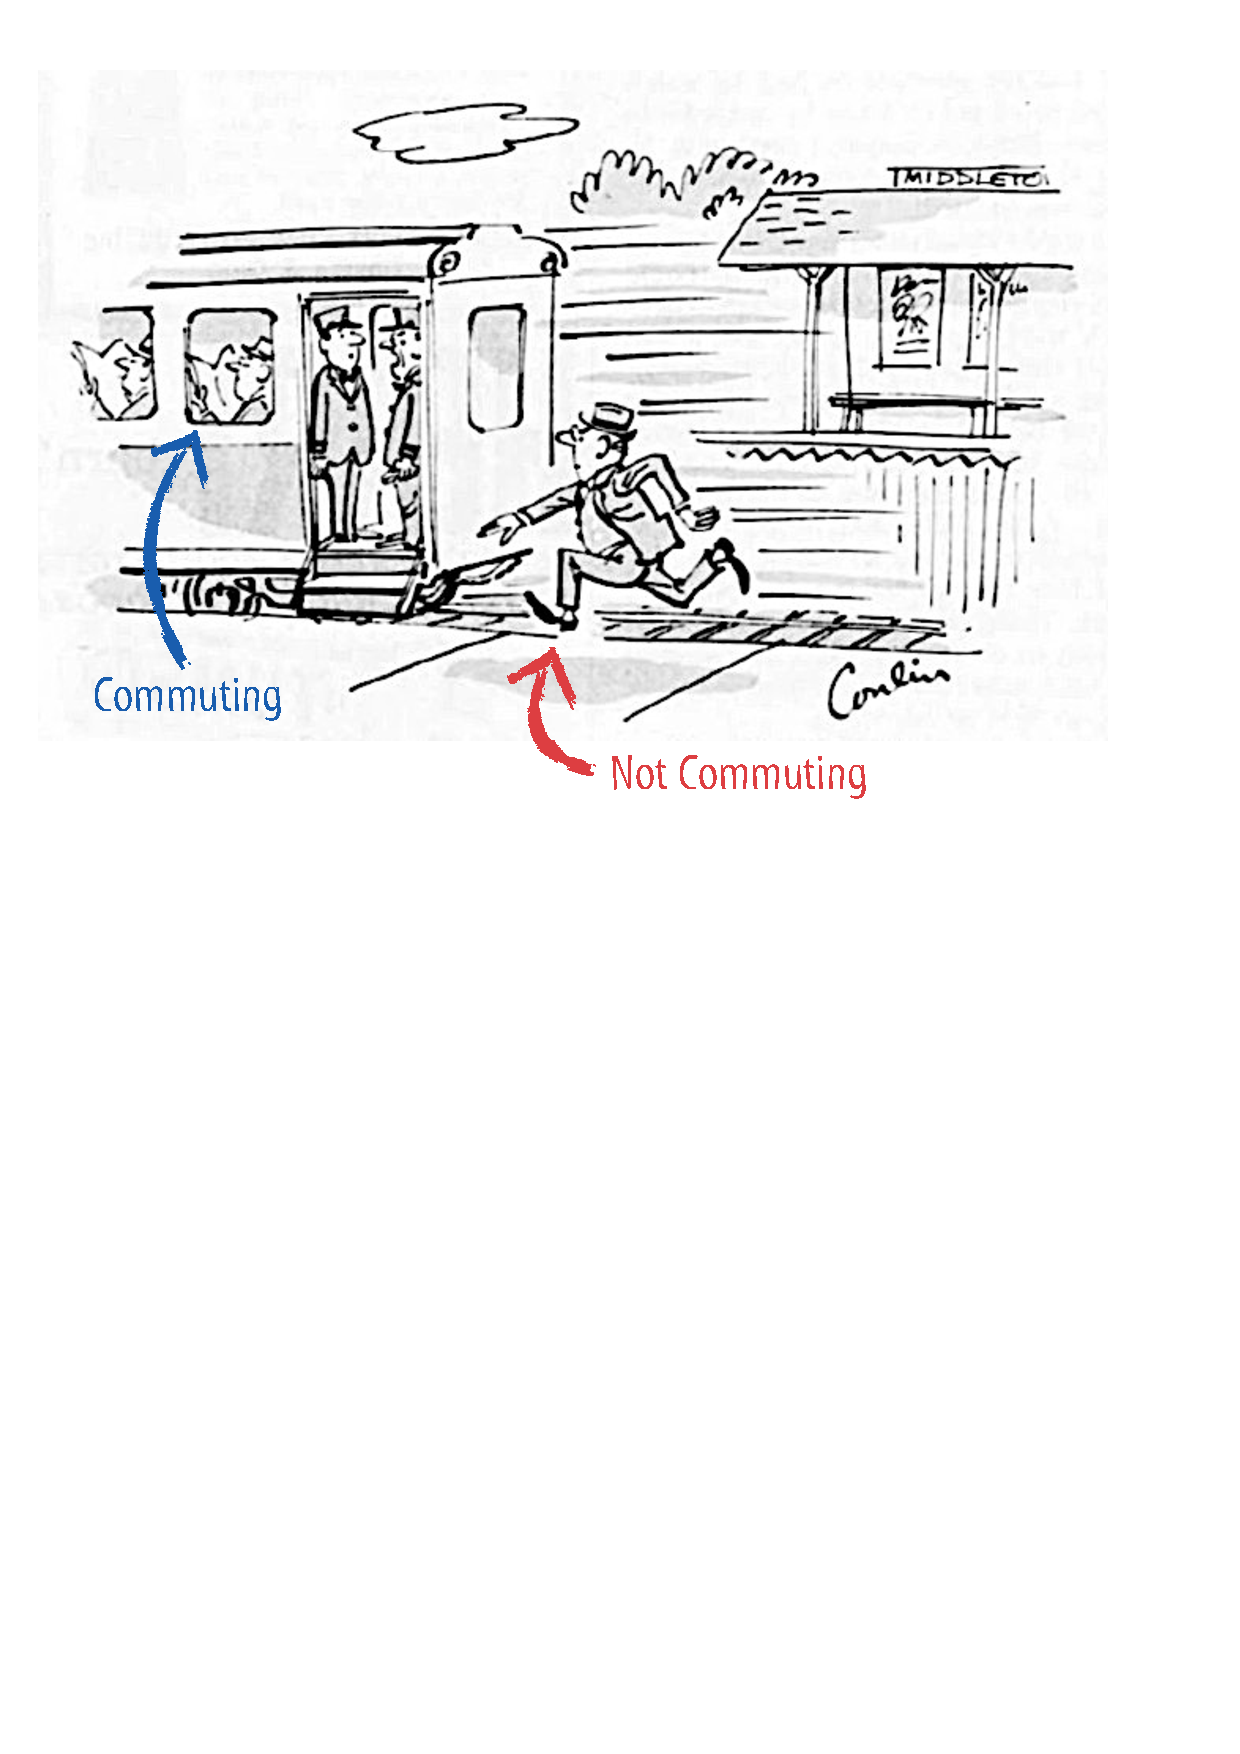
\includegraphics[width=.65\textwidth]{Figures/Commuting.pdf}}
